\documentclass[10pt,a4paper]{article}
\usepackage[utf8]{inputenc}
\usepackage[english]{babel}
\usepackage{amsmath}
\usepackage{amsfonts}
\usepackage{amssymb}
\usepackage{graphicx}
\usepackage[margin=0.5in]{geometry}
\usepackage{amsthm}
\usepackage{enumitem}
\usepackage{tikz}
\newtheorem{question}{Question}
\newtheorem*{question*}{Question}
\newtheorem{theorem}{Theorem}
\newtheorem{lemma}{Lemma}

\theoremstyle{definition}
\newtheorem{answer}{Answer}
\newtheorem*{answer*}{Answer}


\title{Complex Analysis Homework 2}
\author{Colin Williams}

\begin{document}
\maketitle
\section*{Question 4}
\begin{question*}{$ $}
\\Geometrically describe the following subsets of $\mathbb{C}$:
\begin{enumerate}[label = \alph*.)]
\item $|z - i| < |z - 1|$
\item $|z + 2i| \geq 2$
\item $1 < Re(z) \leq 2$
\item $Re(z) \neq 0$.
\end{enumerate}
\end{question*}

\begin{answer*}{\textbf{a.)}}
\\If we first rewrite the inequality as $|z - (0 + i)| < |z - (1 + 0i)|$, then geometrically, the above inequality is the set of all points $z$ such that $z$ is closer to $0 + i$ than it is to $1 + 0i$. Next, express $z$ as $z = x + iy$ and notice the distance described is equal when along the line $y = x$; thus, the inequality is satisfied whenever $y > x$. We can verify this statement algebraically by making the substitution $z = x + iy$ into the given inequality:
\begin{align*}
|z - i| &< |z - 1|\\
|x + iy - i| &< |x + iy - 1|\\
|x + i(y - 1)| &< |(x - 1) + iy|\\
|x + i(y - 1)|^2 &< |(x - 1) + iy|^2\\
x^2 + (y-1)^2 &< (x-1)^2 + y^2\\
x^2 - (x-1)^2 &< y^2 - (y-1)^2\\
x^2 - (x^2 - 2x +1) &< y^2 - (y^2 - 2y +1)\\
2x - 1 &< 2y - 1\\
x &< y
\end{align*}
Thus, we arrive at the same conclusion as we did before: all points $z = x + iy$ satisfy the inequality whenever $y > x$. On a graph, this is represented as:

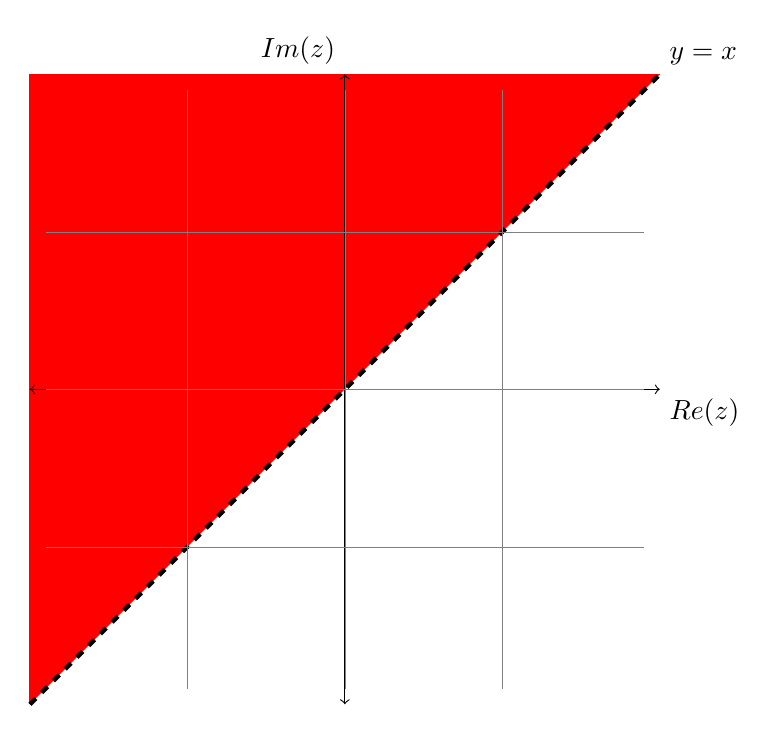
\begin{tikzpicture}[scale = 2]
\draw [fill, red] (-2,-2) -- (-2,2) -- (2,2);
\draw [ultra thick, dashed, black] (-2,-2) -- (2,2);
\draw [<->] (-2,0) -- (2,0);
\node [below right] at (2,0) {$Re(z)$};
\draw [<->] (0,-2) -- (0,2);
\node [above left] at (0,2) {$Im(z)$};
\draw [help lines] (-1.9,-1.9) grid (1.9,1.9);
\node [above right] at (2,2) {$y = x$};
\end{tikzpicture}

\end{answer*}

\begin{answer*}{\textbf{b.)}}
\\First, it may be useful to rewrite this inequality as $|z - (0-2i)| \geq 2$. In this form, it is clear that we are looking for all points $z$ such that the distance between $z$ and $0 - 2i$ is greater than or equal to a distance of 2. Intuitively, this would be the set of all points on the boundary and outside of a circle of radius 2 centered at $0 - 2i$. Again, let's verify this algebraically by plugging $z = x+iy$ into the inequality:
\begin{align*}
|z + 2i| &\geq 2\\
|x + iy + 2i| &\geq 2\\
|x + i(y+2)| &\geq 2\\
|x + i(y+2)|^2 &\geq 2^2\\
x^2 + (y+2)^2 &\geq 2^2
\end{align*}

This verifies that the first inequality describes precisely what I claimed: the set of all points $z$ outside of or on the border of the circle of radius 2 centered at $0 - 2i$. Graphically, this is represented as:

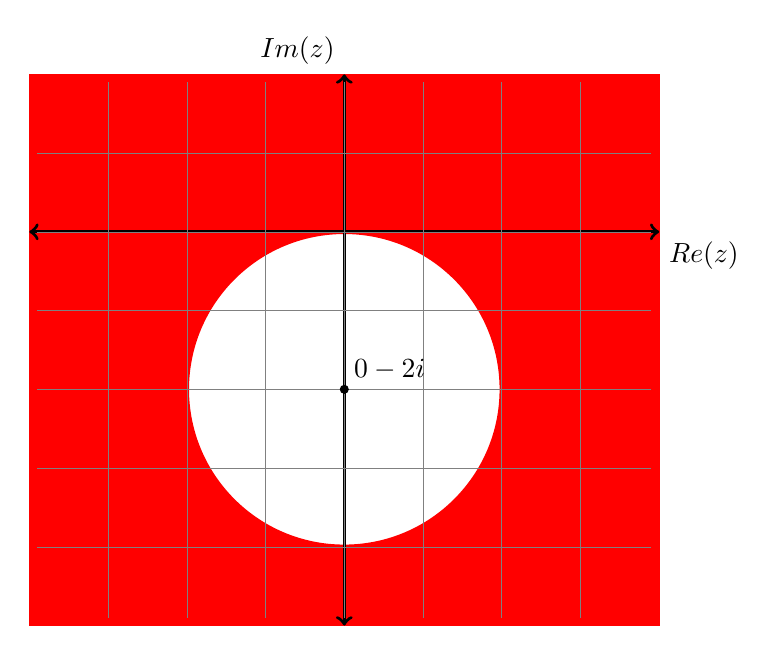
\begin{tikzpicture}[scale = 1]
\draw [fill, red] (-4,-5) -- (-4,2) -- (4,2) -- (4,-5);
\draw [fill, white] (0,-2) circle [radius = 2];
\draw [ultra thick, red] (0,-2) circle [radius = 2];
\draw [<->, very thick] (-4,0) -- (4,0);
\node [below right] at (4,0) {$Re(z)$};
\draw [<->, very thick] (0,-5) -- (0,2);
\node [above left] at (0,2) {$Im(z)$};
\draw [help lines] (-3.9,-4.9) grid (3.9,1.9);
\draw [fill, black] (0,-2) circle [radius = 0.05];
\node [above right] at (0,-2) {$0 - 2i$};
\end{tikzpicture}

\end{answer*}

\begin{answer*}{\textbf{c.)}}
\\If we write $z$ as $z = x + iy$, then it is clear that $Re(z) = x$. Thus, the given inequality is also expressed as $1 < x \leq 2$. Geometrically, this is a vertical strip on the complex plane with the left side of the strip not included at $x = 1$, and the right side of the strip included at $x = 2$. On a graph, this looks like:

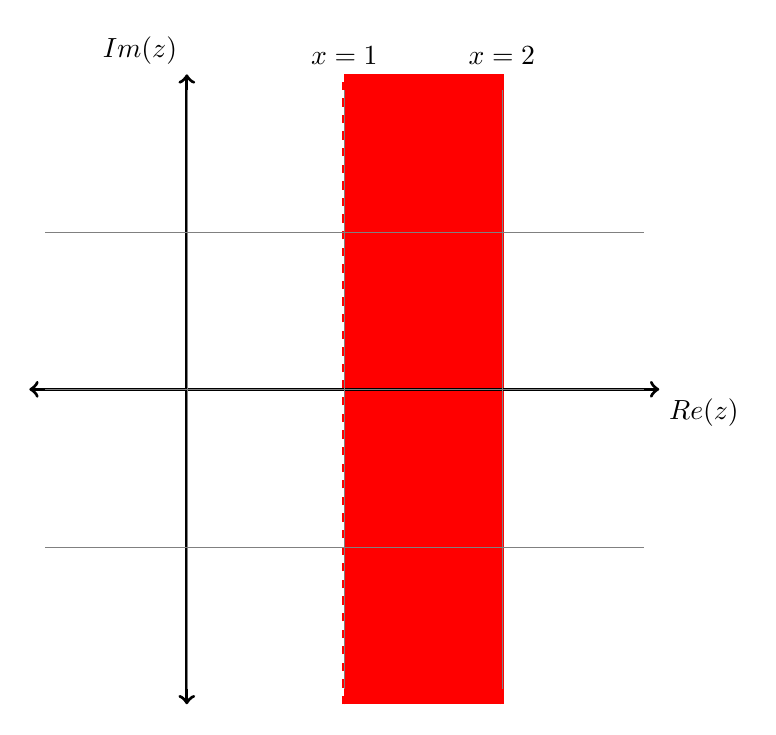
\begin{tikzpicture}[scale = 2]
\draw [fill, red] (1,-2) -- (1,2) -- (2,2) -- (2,-2);
\draw [ultra thick, dashed, red] (1,-2) -- (1,2);
\draw [ultra thick, red] (2,-2) -- (2,2);
\draw [<->, very thick] (-1,0) -- (3,0);
\node [below right] at (3,0) {$Re(z)$};
\draw [<->, very thick] (0,-2) -- (0,2);
\node [above left] at (0,2) {$Im(z)$};
\draw [help lines] (-.9,-1.9) grid (2.9,1.9);
\node [above] at (1,2) {$x = 1$};
\node [above] at (2,2) {$x = 2$};
\end{tikzpicture}

\end{answer*}

\begin{answer*}{\textbf{d.)}}
\\The above statement represents all points on the complex plane expect those where $Re(z) = 0$. If we write $z$ as $z = x+iy$, then this is equivalent to all points except where $x = 0$. Graphically, this can be represented by:

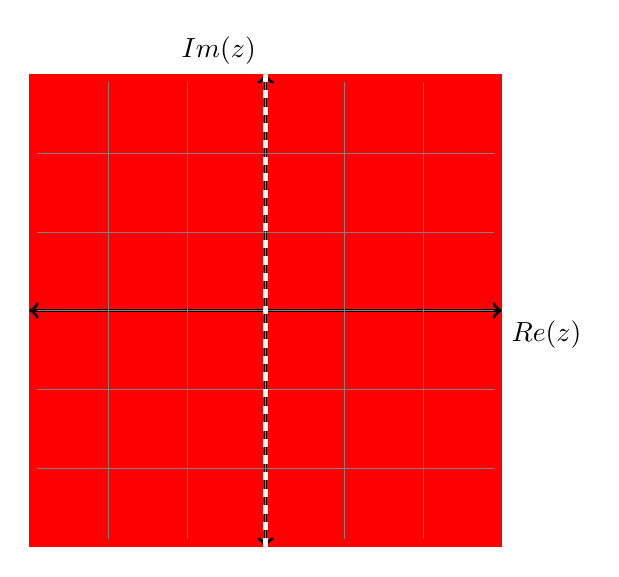
\begin{tikzpicture}[scale = 1]
\draw [fill, red] (-3,-3) -- (-3,3) -- (3,3) -- (3,-3);
\draw [<->, very thick] (-3,0) -- (3,0);
\node [below right] at (3,0) {$Re(z)$};
\draw [<->, very thick] (0,-3) -- (0,3);
\node [above left] at (0,3) {$Im(z)$};
\draw [help lines] (-2.9,-2.9) grid (2.9,2.9);
\draw [ultra thick, dashed, white] (0,-3) -- (0,3);
\end{tikzpicture}

\end{answer*}

\end{document}